\documentclass[11pt,letterpaper]{article}
\usepackage[margin=1.0in]{geometry}
\usepackage[utf8]{inputenc}
\usepackage{cite}
\usepackage{amsmath}
\usepackage{amsfonts}
\usepackage{amssymb}
\usepackage{makeidx}
\usepackage{graphicx}
\usepackage{hyperref}
\setlength\parindent{0pt}

\author{STUDENT NAME}
\title{Lab1: Circuit Analysis}

\begin{document}

\maketitle

\section{Objectives}

\begin{enumerate}
\item To understand how to read resistor values using the color coding system
\item To measure the true value of resistors using a handheld Digital Multimeter (DMM)
\item To build a simple resistor circuit using a standard breadboard
\item To measure voltage drops across resistors using the DMM
\item To measure current flowing in a branch
\item To understand why measuring voltages is safe, since the internal resistance of the meter in that setting is near infinite (at least $10^7 \Omega$ or 10 MegaOhm  )
\item To understand why measuring current can be dangerous, since the internal resistance of the meter in that setting is zero, and shortcuts can be easily made.
\item To understand and verify the three basic circuit laws being i) Ohm’s Law, ii) Kirchoff’s Voltage Law (KVL) and iii) Kirchoff’s Current Law (KCL)
\end{enumerate}

\section{Equipment}

\begin{enumerate}
\item Power supply
\item Bread board
\item Resistors, 1k, 2.7k, 4.7k, 10k
\item Handheld Digital Multimeter (DMM)
\end{enumerate}

\section{Procedures}

Measure the exact values of the resistors using the handheld DMM, and determine the color coding of the resistors using Figure \ref{fig:Lab1_ResistorColorCoding} and Figure \ref{fig:Lab1_ResistorColorCodingTable}. To determine the value of a resistor use the following equation: $R = ab * 10^c \pm d \% $. Example: If a resistor has the color coding Yellow-Violet-Red-Gold, then $a$ = 4, $b$ = 7, $c$ = 2 and $d$ = 5 \%. The value of the resistor is now $47 * 10^2 = 4.7k \pm 5 \%$. Fill out the following table:
\begin{center}
\begin{tabular}{|c|c|c|c|c|c|}
\hline Nominal value & Measured value  & Color ring 1  & Color ring 2 & Color ring 3 & Tolerance \\ 
\hline 1k &  &  &  &  &  \\ 
\hline 2.7k  &  &  &  &  &  \\ 
\hline 4.7k &  &  &  &  &  \\ 
\hline 10k &  &  &  &  &  \\ 
\hline 
\end{tabular}
\end{center}

The breadboard is organized as shown in Figure \ref{fig:Lab1_BreadBoard}: There are three binding posts, on which we will connect the 10 V DC power supply (positive is red, ground is black).\\

\begin{figure}
\centering
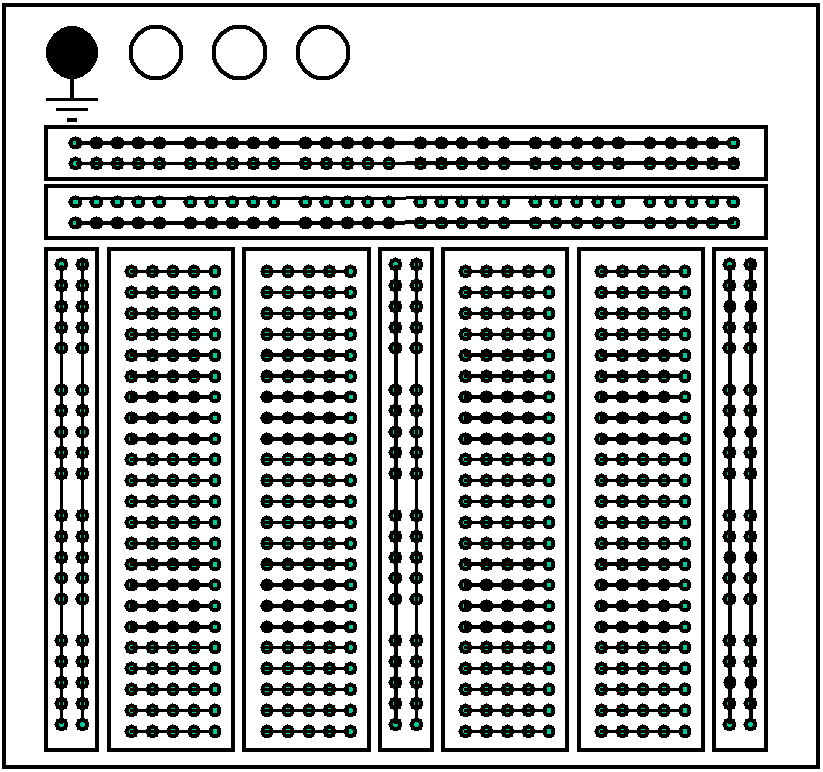
\includegraphics[width=0.5\linewidth]{Lab1_BreadBoard}
\caption{Typical bread board for experimental circuit construction.}
\label{fig:Lab1_BreadBoard}
\end{figure}

\begin{figure}
\centering
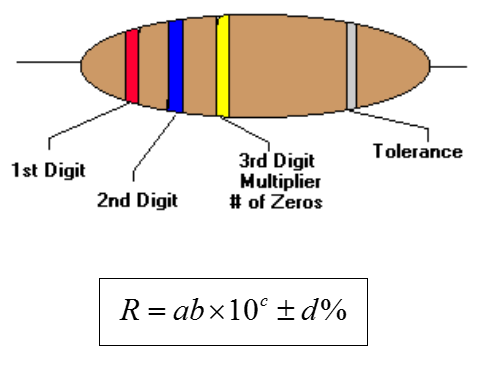
\includegraphics[width=0.8\linewidth]{Lab1_ResistorColorCoding}
\caption{Resistor Color Coding Chart. }
\label{fig:Lab1_ResistorColorCoding}
\end{figure}

\begin{figure}
\centering
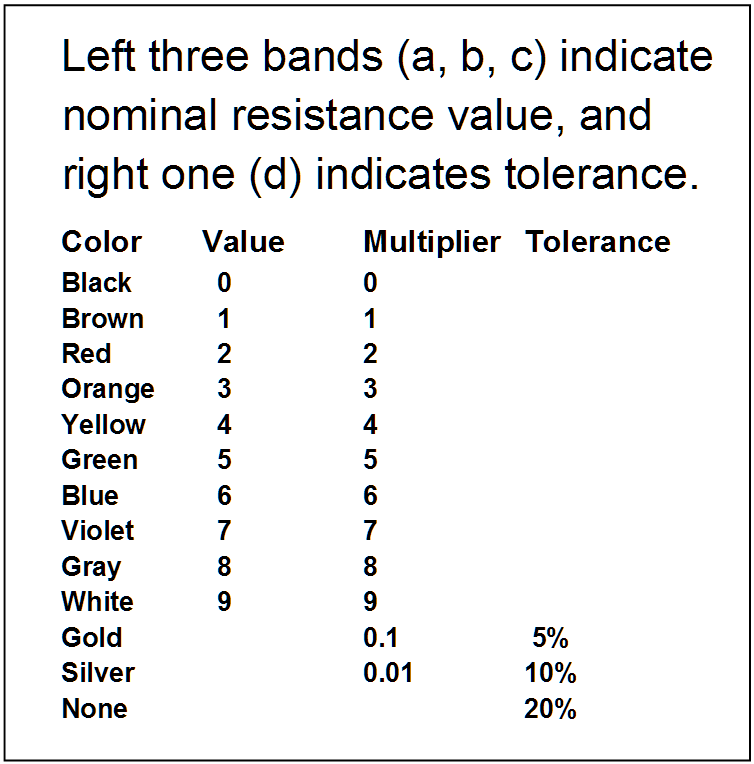
\includegraphics[width=0.6\linewidth]{Lab1_ResistorColorCodingTable}
\caption{Resistor Color Coding Table.}
\label{fig:Lab1_ResistorColorCodingTable}
\end{figure}

\section{Circuit measurements}	

1) Hook up the circuit as shown below on the breadboard. When you are done, let the TA or instructor check your work.\\
2) Turn on the power supply with the input dials all the way down (CCW) and slowly adjust the power supply to 10V.\\

\begin{figure}
\centering
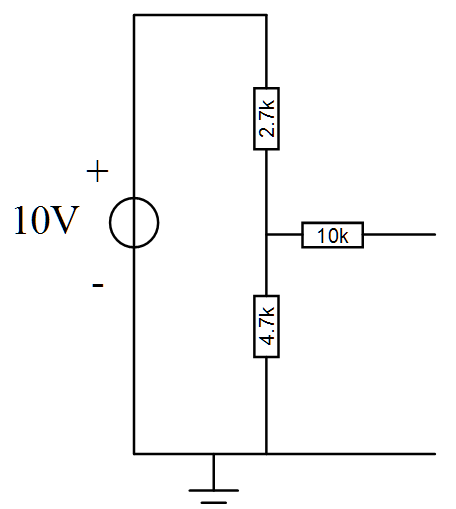
\includegraphics[width=0.5\linewidth]{Lab1_Circuit1}
\caption{Circuit1. Ask yourself how much current is flowing in the 10k branch.}
\label{fig:Lab1_Circuit1}
\end{figure}

3) Measure the voltages across all resistors as shown in Figure \ref{fig:Lab1_Circuit1}; keep the red DMM wire on top. Fill out the table:

\begin{center}
\begin{tabular}{|c|c|}
\hline Nominal value & Voltage drop (V)\\ 
\hline 2.7k &  \\ 
\hline 4.7k &  \\ 
\hline 10k &  \\ 
\hline 
\end{tabular} 
\end{center}

\begin{center}
VOLTAGE MEASUREMENTS ARE SAFE, SINCE IN THIS MODE THE INTERNAL RESISTANCE OF THE METER IS NEAR INFINITE.
\end{center}

4) Measure the current flowing into the 2.7k resistor as shown in Figure \ref{fig:Lab1_Circuit2}\\ 

\begin{figure}
\centering
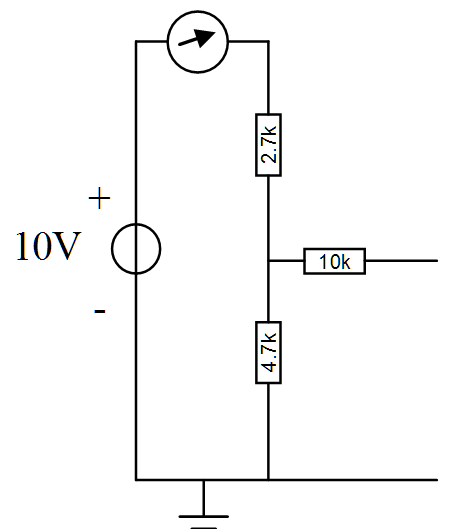
\includegraphics[width=0.5\linewidth]{Lab1_Circuit2}
\caption{Circuit2. Measure the current into the 2.7k resistor, after the measurement set your DVM back to Voltage measurement.}
\label{fig:Lab1_Circuit2}
\end{figure}

\begin{center}
CURRENT MEASUREMENTS ARE POTENTIALLY DANGEROUS BECAUSE IN THIS MODE THE INTERNAL RESISTANCE OF THE METER IS ZERO, SO PAY CLOSE ATTENTION.\\
\end{center}

4a) Remove the top wire of the 2.7k resistor\\
4b) Turn your DMM to Current measurement and move the red wire to Current Measurement\\
4c) Connect your meter between the positive binding post and the loose end of the resistor\\
4d) Measure the current and fill out the table:\\

\begin{center}
\begin{tabular}{|c|c|}
\hline Nominal value & Current (A)\\ 
\hline 2.7k &  \\ 
\hline 
\end{tabular} 
\end{center}


4e) \textbf{Immediately move the red wire of the DMM back to Voltage measurement and turn the dial to DC Voltage measurement.} Measure the voltage drops across the following resistors and fill out the table.\\

\begin{center}
\begin{tabular}{|c|c|}
\hline Nominal value & Voltage drop (V)\\ 
\hline 2.7k &  \\ 
\hline 4.7k &  \\ 
\hline 10k &  \\ 
\hline 
\end{tabular} 
\end{center}

5) Repeat the voltage measurements with the 1k resistor placed in series with the 10k resistor as shown in Figure \ref{fig:Lab1_Circuit3}. Fill out the table:\\

\begin{figure}
\centering
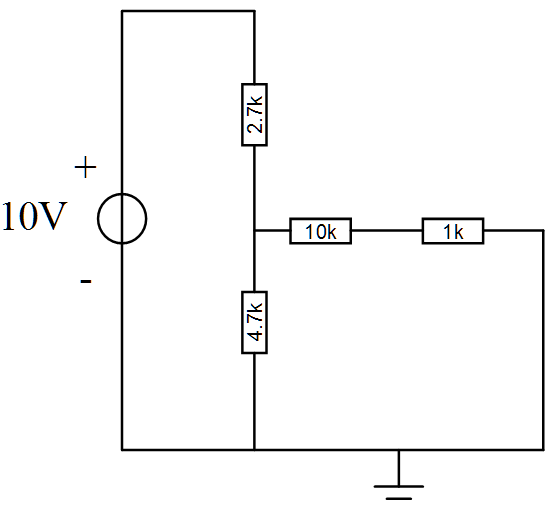
\includegraphics[width=0.6\linewidth]{Lab1_Circuit3}
\caption{Circuit3. Connect a 1k resistor in series with the 10k resistor. Measure the voltages across all resistors.}
\label{fig:Lab1_Circuit3}
\end{figure}

\begin{center}
\begin{tabular}{|c|c|}
\hline Nominal Value & Voltage drop (V)  \\ 
\hline 2.7k &  \\ 
\hline 4.7k &  \\ 
\hline 10k &  \\ 
\hline 1k &  \\ 
\hline 
\end{tabular} 
\end{center}

6) Measure the current flowing into the 1k resistor, the 4.7k resistor and into the 10k+1k branch as shown in Figure \ref{fig:Lab1_Circuit4}. Fill out the table:

\begin{figure}
\centering
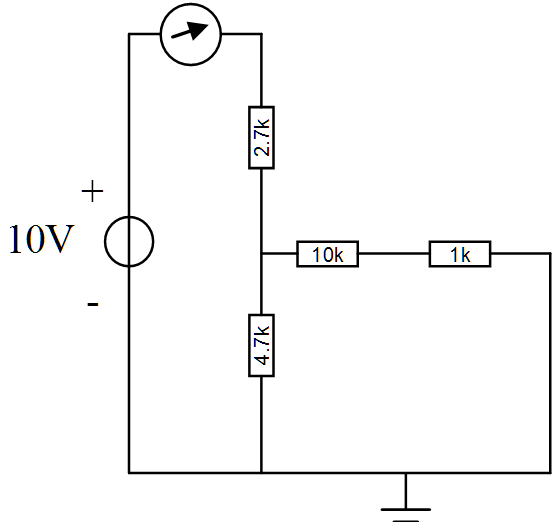
\includegraphics[width=0.6\linewidth]{Lab1_Circuit4}
\caption{Circuit4. Measure the current into the 2.7k resistor, the 4.7k resistor and the branch containing the 10k and 1k resistor. After the measurement set your DVM back to Voltage measurement.}
\label{fig:Lab1_Circuit4}
\end{figure}

\begin{center}
\begin{tabular}{|c|c|}
\hline Nominal value & Current (A)\\ 
\hline 2.7k &  \\ 
\hline 4.7k &  \\ 
\hline 10k+1k &  \\ 
\hline 
\end{tabular} 
\end{center}

\section{Questions}

Q1: Using Ohm’s law $\Delta U = i R$ verify the measured values of the voltages across all resistors

\begin{equation} \label{Eqn:LabIntroduction1}
\Delta U = i R
\end{equation}

A1:\\


Q2: Show the validity of Kirchhoff’s voltage law which reads: In a closed loop, the algebraic sum of the voltages must be zero. To do this, in the closed loop 4.7k – 10k – 1k measure all voltages keeping the order of polarity the same (always measure high-low or red wire/black wire) and add them up.\\

A2:\\


Q3: Show the validity of Kirchoff’s current law which reads: In a node, the algebraic sum of the currents must be zero. Verify this using the current measurements from section 6).\\

A3:\\


\section{Links}

\href{http://en.wikipedia.org/wiki/Ohm%27s_law}{Ohm's Law}\\
\href{http://en.wikipedia.org/wiki/Kirchhoff%27s_circuit_laws}{Kirchoff's Laws}

\end{document}

